\documentclass[a4paper,12pt]{article}

\usepackage[table]{xcolor}%TABLAS
\usepackage{booktabs}
\usepackage{multirow}
\usepackage{colortbl}
\usepackage[hypcap=false, font=small]{caption}
\usepackage{multicol}%poder colocar columnas
\usepackage{amsmath} %formulas
\usepackage{amssymb} %simbolos
\usepackage{amsfonts} 
\usepackage{array}
\usepackage{verbatim}%escribir sin codigos y comentarios multilinea
\usepackage{xcolor}%cambiar el color del texto
\usepackage{siunitx}%unidades del sistema internacional
\usepackage{subcaption}%leyendas en objetos que tienen su leyenda
\usepackage{fancyhdr}%personalizar encabezado y pie de pagina
\usepackage{longtable}%crear tablas largas
\usepackage{hyperref}%crear e insertar links
\usepackage[utf8]{inputenc} %facilitar la escritura en español 
\usepackage{graphicx}% figuras
\usepackage[spanish,es-tabla]{babel} %tipografia del idioma
%\usepackage{biblatex}%bibliografia automatica apartir de base bib
\usepackage{blindtext}%texto de relleno
\usepackage{grffile}
\usepackage{mathrsfs}
\usepackage{multirow}
\usepackage{siunitx}
\usepackage{soul}%subrayar

\graphicspath{{./Fotos}}

\newenvironment{Figure}
  {\par\medskip\noindent\minipage{\linewidth}}
  {\endminipage\par\medskip}

\usepackage{anysize}
\marginsize{2cm}{2cm}{1cm}{2cm}

\setlength\columnsep{18pt}
\setlength\parskip{4pt} \setlength\parindent{0in}

\title{Formación de imágenes por refracción con lentes \\ 
\medskip \large Universidad Nacional de Tucumán}
\author{Iker Algañaraz, May Juarez F., Gastón A. Lozano S., Belén N. Paz}
\date{}

\begin{document}

\maketitle

\section*{Resumen}

    En este informe se comprobó la aplicabilidad del modelo que relaciona la distancia imagen de una lente con la distancia objeto, tanto para lentes convergentes como para lentes divergentes. Se controló además los supuestos del modelo, como las aberraciones cromáticas y esféricas, y se concluyó que era aplicable en ambos casos.

\medskip

\begin{multicols*}{2}

\section*{Introducción}

    La formación de imágenes con lentes es un fenómeno óptico fundamental que desempeña un papel crucial en una amplia variedad de aplicaciones, desde la fotografía hasta la medicina y la astronomía. Este informe se sumerge en los principios matemáticos y físicos que rigen la formación de imágenes con lentes.

\section*{Marco teórico}

    Los lentes delgados son un caso especial de lentes en el que su grosor es despreciable en comparación a las longitudes asociadas con sus propiedades ópticas, tales como la distancia objeto, la distancia imagen, y los radios de curvatura. Una propiedad de los lentes, que difiere de los espejos, son sus dos puntos focales uno a cada lado, ya que por ambos pasa luz. Además, en las lentes delgadas, estos puntos se encuentran a distancias iguales medidas desde su centro.

    A partir de relaciones de triángulos congruentes al realizar los diagramas de rayos, es posible encontrar una relación de las longitudes asociadas a las propiedades ópticas, obteniendo la ecuación:
    
    \begin{equation} 
        \label{eq:1/i+1/o}
        \frac{1}{o}+\frac{1}{i}=\frac{1}{f}
    \end{equation}

    Donde \textit{o} es la distancia objeto, \textit{i} es la distancia imagen, y \textit{f} es la distancia focal. Esta relación es válida para lentes delgadas y rayos paraxiales, es decir, aquellos cuyo ángulo con respecto al eje es pequeño. Es posible determinar otra relación entre la distancia objeto, el índice de refracción y los radios de curvaturas, conocida como la \textit{ecuación del fabricante}:

    \begin{equation*}
        (n-1) \left(\frac{1}{R_{1}}-\frac{1}{R_{2}} \right)=\frac{1}{f}
    \end{equation*}

    Donde $R_{1}$ y $R_{2}$ son los radios de curvatura de los lentes. Esta relación, al igual que (\ref{eq:1/i+1/o}) es válida para rayos paraxiales, ya que para aquellos que formen ángulos grandes con el eje no convergen en el mismo punto.

    Si se conoce la distancia focal y la posición del objeto, es posible encontrar la posición de su imagen por tres métodos: diagrama de rayos (figura \ref{Diag rayos LC} y \ref{f: rayos LD}), experimentalmente, o utilizando la ecuación (\ref{eq:1/i+1/o}).

    Estos lentes se clasifican en dos tipos: \textbf{convergentes} y \textbf{divergentes}. Cuando un haz de rayos paralelos al eje óptico (recta que pasa por el centro geométrico de la lente y es perpendicular a sus dos caras) se refracta al pasar por la lente convergente, en una situación ideal, se dirigen al punto focal del lado opuesto por el que ingresaron, como se muestra en la figura \ref{rayos LC}, siendo $F_{1}$ y $F_{2}$ los puntos focales y \emph{f} la distancia focal (siempre positiva en lentes convergentes). Si por lo contrario, el haz de rayos diverge de $F_{1}$ e incide en la lente, al refractarse será paralelo al eje. De la figura \ref{rayos LC} se observa que los lentes convergentes son más gruesos en el centro y menos en sus bordes.

    \begin{Figure}
        \centering
        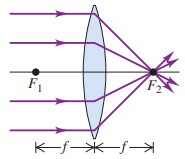
\includegraphics[width=0.6\linewidth]{LenteConvergente1.jpg}
        \captionof{figure}{Lente convergente}
        \label{rayos LC}
    \end{Figure}

    Los lentes divergentes se caracterizan por ser más gruesos en sus bordes que en su centro. Al ser atravesados por un haz de rayos paralelos al eje óptico, emergen de la lente como si divergieran de $F_{2}$ (Fig. \ref{Rayos LD}). Si los rayos incidentes parecieran converger al punto focal $F_{1}$, al refractarse se dirigirán paralelamente al eje óptico.

    \begin{Figure}
        \centering
        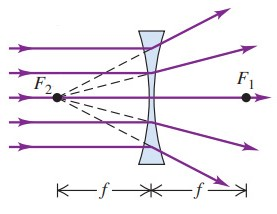
\includegraphics[width=0.7\linewidth]{Rayos LD.jpg}
        \captionof{figure}{Lente divergente}
        \label{Rayos LD}
    \end{Figure}

    \subsection*{Formación de imágenes en una lente convergente}

        Las imágenes formadas cuando la distancia objeto es mayor que la distancia focal son reales, siendo posible recogerlas en una pantalla. Al colocar un objeto en uno de los lados del lente, su imagen se formará  del lado opuesto a este, como se muestra en la figura \ref{Diag rayos LC}a, la imagen es invertida y más pequeña. Si la distancia objeto es menor que la distancia focal, la imagen que se forma es virtual, siendo imposible recogerla con una pantalla (la imagen se construye a partir de la prolongación de los rayos refractados), como se muestra en la figura \ref{Diag rayos LC}b, la imagen es derecha y más grande.

        % Diagrama de rayos LC
        \begin{Figure}
            \centering
            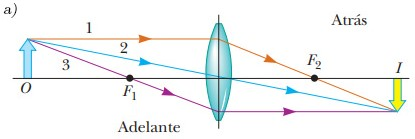
\includegraphics[width=1\linewidth]{Diagrama de rayos LC 1.jpg}
        \end{Figure}

        \begin{Figure}
            \centering
            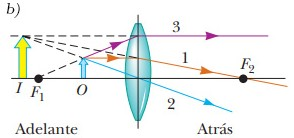
\includegraphics[width=0.7\linewidth]{Diagrama de rayos LC 2.jpg}
            \captionof{figure}{Diagrama de rayos, lente convergente}
            \label{Diag rayos LC}
        \end{Figure}

       En la figura se muestran rayos que divergen de un punto del objeto. Para simplificar el diagrama, se trazan 3 rayos principales:

        \begin{enumerate}
            \item Rayo paralelo al eje emerge de la lente y pasa por el punto focal $F_{2}$.
            \item Rayo que pasa por el centro de la lente, la desviación no es apreciable por lo que sigue una línea recta.
            \item Rayo que pasa por el punto focal $F_{1}$ y emerge paralelo al eje.
        \end{enumerate}

    \subsection*{Formación de imágenes en una lente divergente}

        La distancia focal en las lentes divergentes es siempre negativa, es decir, se forman imágenes virtuales independientemente de la posición del objeto. Esta imagen es siempre de menor tamaño y próxima al lente, como se muestra en la figura \ref{f: rayos LD}.

        % Diagrama de rayos LD
        \begin{Figure}
            \centering
            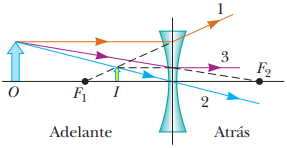
\includegraphics[width=0.9\linewidth]{Diag de rayos LD.png}
            \captionof{figure}{Diagrama de rayos, lente divergente}
            \label{f: rayos LD}
        \end{Figure}

        Al igual que la figura \ref{Diag rayos LC}, se trazan 3 rayos:

        \begin{enumerate}
            \item Rayo paralelo al eje que al refractarse por la lente parece provenir del punto focal $F_{1}$, se aleja de $F_{2}$.
            \item Rayo que pasa por el centro de la lente, la desviación no es apreciable por lo que sigue una línea recta.
            \item Rayo con dirección de $F_{2}$ que al refractarse emerge de la lente paralelo al eje.
        \end{enumerate}

    \subsection*{Aberraciones}

        En una situación ideal, la imagen de una lente es nítida, sin embargo en la realidad esto no sucede. Se debe a que no todos los rayos son paraxiales, por lo que no convergen en el mismo punto de los que sí lo son. Este fenómeno recibe el nombre de \emph{aberración esférica}, ilustrada en la figura \ref{f:abesf}. El punto de convergencia de los rayos paraxiales se encuentra más lejos que aquellos que no lo son, que convergen más cerca de la lente. Es posible reducir la aberración implementando un diafragma, es decir, un orificio por el que se puede controlar la cantidad de luz que entra. Debido a este artefacto, es posible seleccionar una mayor cantidad de rayos paraxiales y en consecuencia obtener una imagen más nítida. Sin embargo una desventaja es la disminución de luz.

        Otro tipo de aberración que se presenta en los lentes es la \emph{aberración cromática}, que se debe a la variación del indice de refracción con respecto de la longitud de onda. Al pasar luz blanca a través de una lente, se refracta de manera que los rayos azules convergen más cerca del lente y los rojos más lejos, mientras que los rayos verdes convergen en un punto intermedio, como se muestra en la figura \ref{f: abcro}.

        %aberraciones
        \begin{Figure}
            \centering
            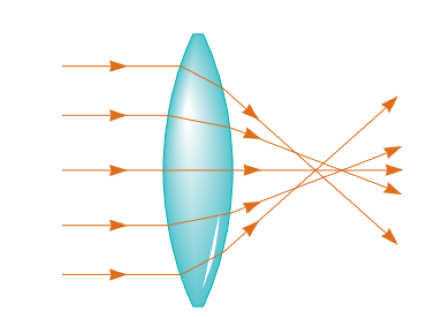
\includegraphics[width=0.7\linewidth]{Aberracion esfericaa.png}
            \captionof{figure}{Aberración esférica}
            \label{f:abesf}
        \end{Figure}

        \begin{Figure}
            \centering
            \includegraphics[width=0.7\linewidth]{ab cromatica.jpg}
            \captionof{figure}{Aberración crómatica}
            \label{f: abcro}
        \end{Figure}

\newpage

\section*{Método experimental}

    \subsection*{Lente convergente}
    
        Con el objetivo de comprobar experimentalmente la relación entre la distancia imagen y la distancia objeto para una lente convergente (\ref{eq:1/i+1/o}), hemos diseñado un sistema experimental a partir del equipo \emph{PASCO Basic Optics System} (figura \ref{PASCOconv}) con el que poder determinar si el modelo es aplicable, y en caso de serlo, usarlo para medir la distancia focal del equipo.

        El sistema experimental consta de un riel milimetrado en el que colocamos una fuente luminosa en la posición 0.0, una lente convergente después de la fuente, y una pantalla detrás de la lente. La distancia objeto (o) es la distancia entre la fuente y la lente, mientras que la distancia imagen (i) será la distancia entre la lente y la pantalla.

        Al momento de usar el sistema experimental, lo que se hará es mover el lente, y ver dónde está la imagen real después del cambio. Si se cumple el modelo, deberíamos de poder ver una relación lineal entre $\frac{1}{i}$ y $\frac{1}{o}$.

        % Diagrama lente convergente
        \begin{Figure}
            \centering
            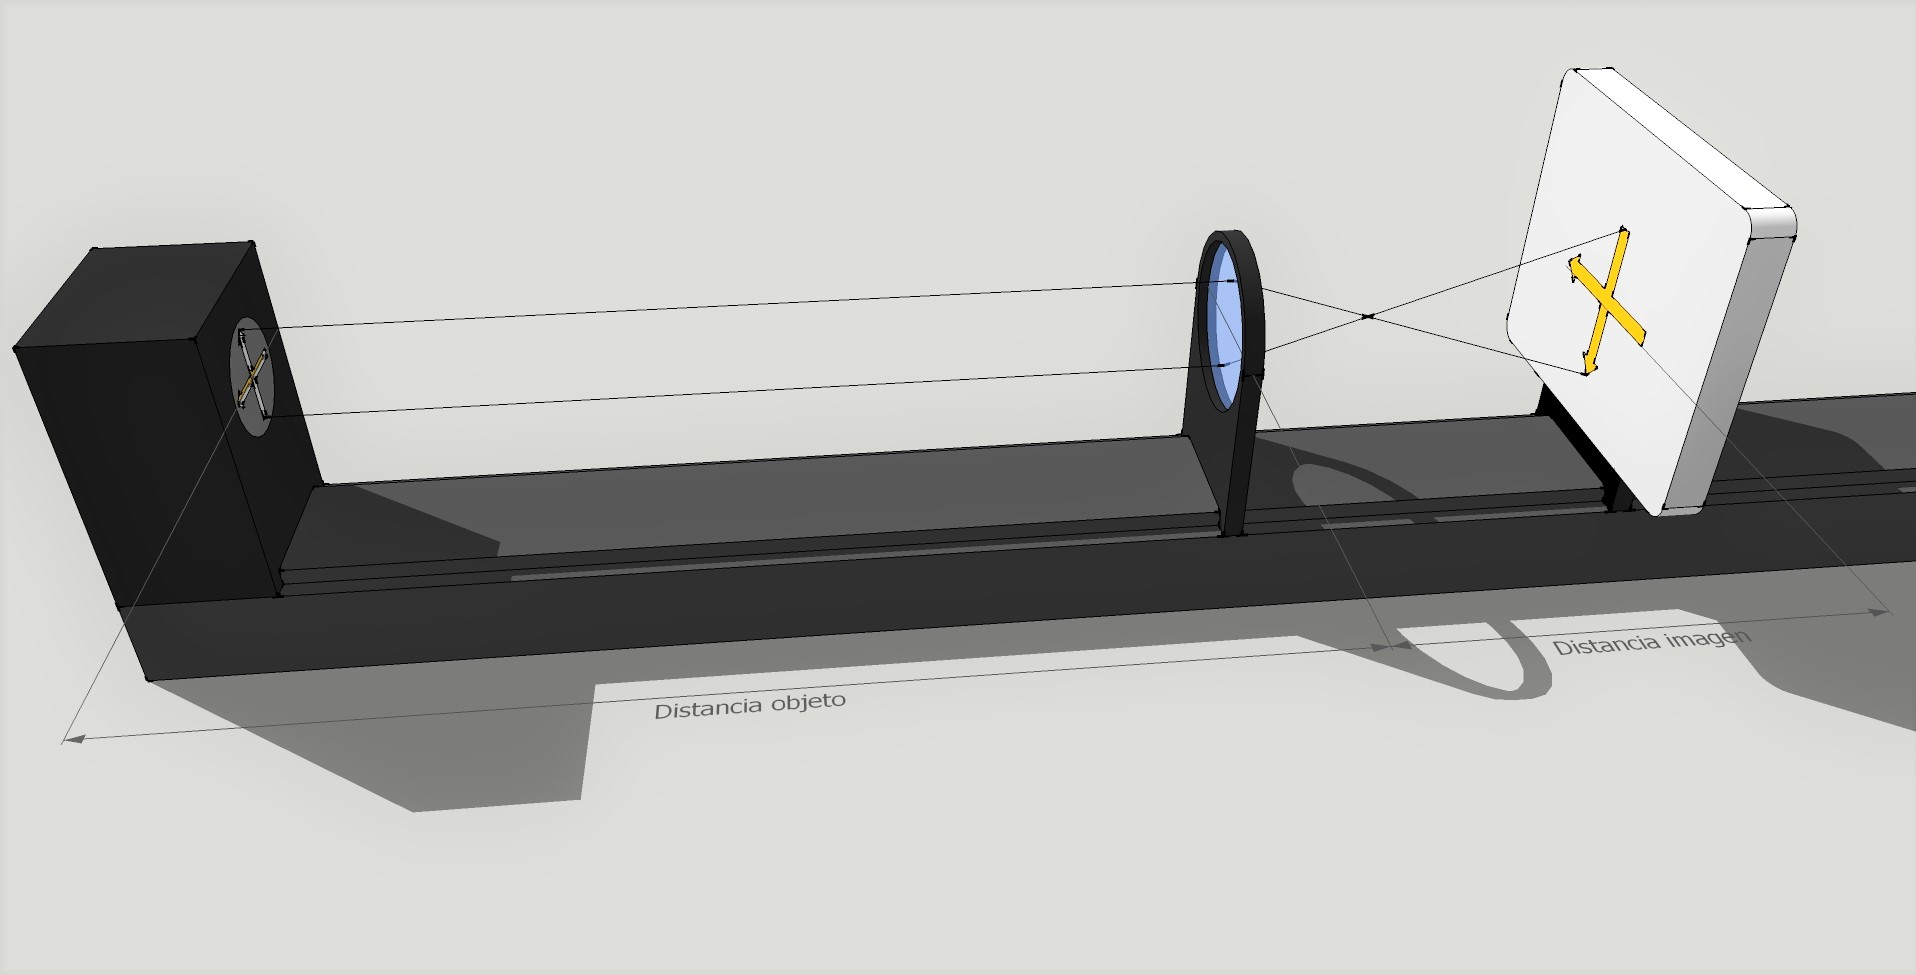
\includegraphics[width=1\linewidth]{Lente convergente.jpg}
            \captionof{figure}{Sistema experimental lente convergente}
            \label{PASCOconv}
        \end{Figure}

    \subsection*{Lente divergente}

        El sistema experimental utilizado para medir las distancias objeto e imagen de una lente divergente fue creado a partir del equipo \emph{PASCO Basic Optics System}, el mismo hace uso de una lente convergente para conseguir rayos que incidan de forma convergente hacia la lente deseada. El diagrama se encuentra en la figura \ref{fig:Diagramaconvex}, como se observa los rayos refractados por la lente divergente logran formar una imagen real cuya distancia es medible experimentalmente.

        % Diagrama Lente divergente
        \begin{Figure}
            \centering
            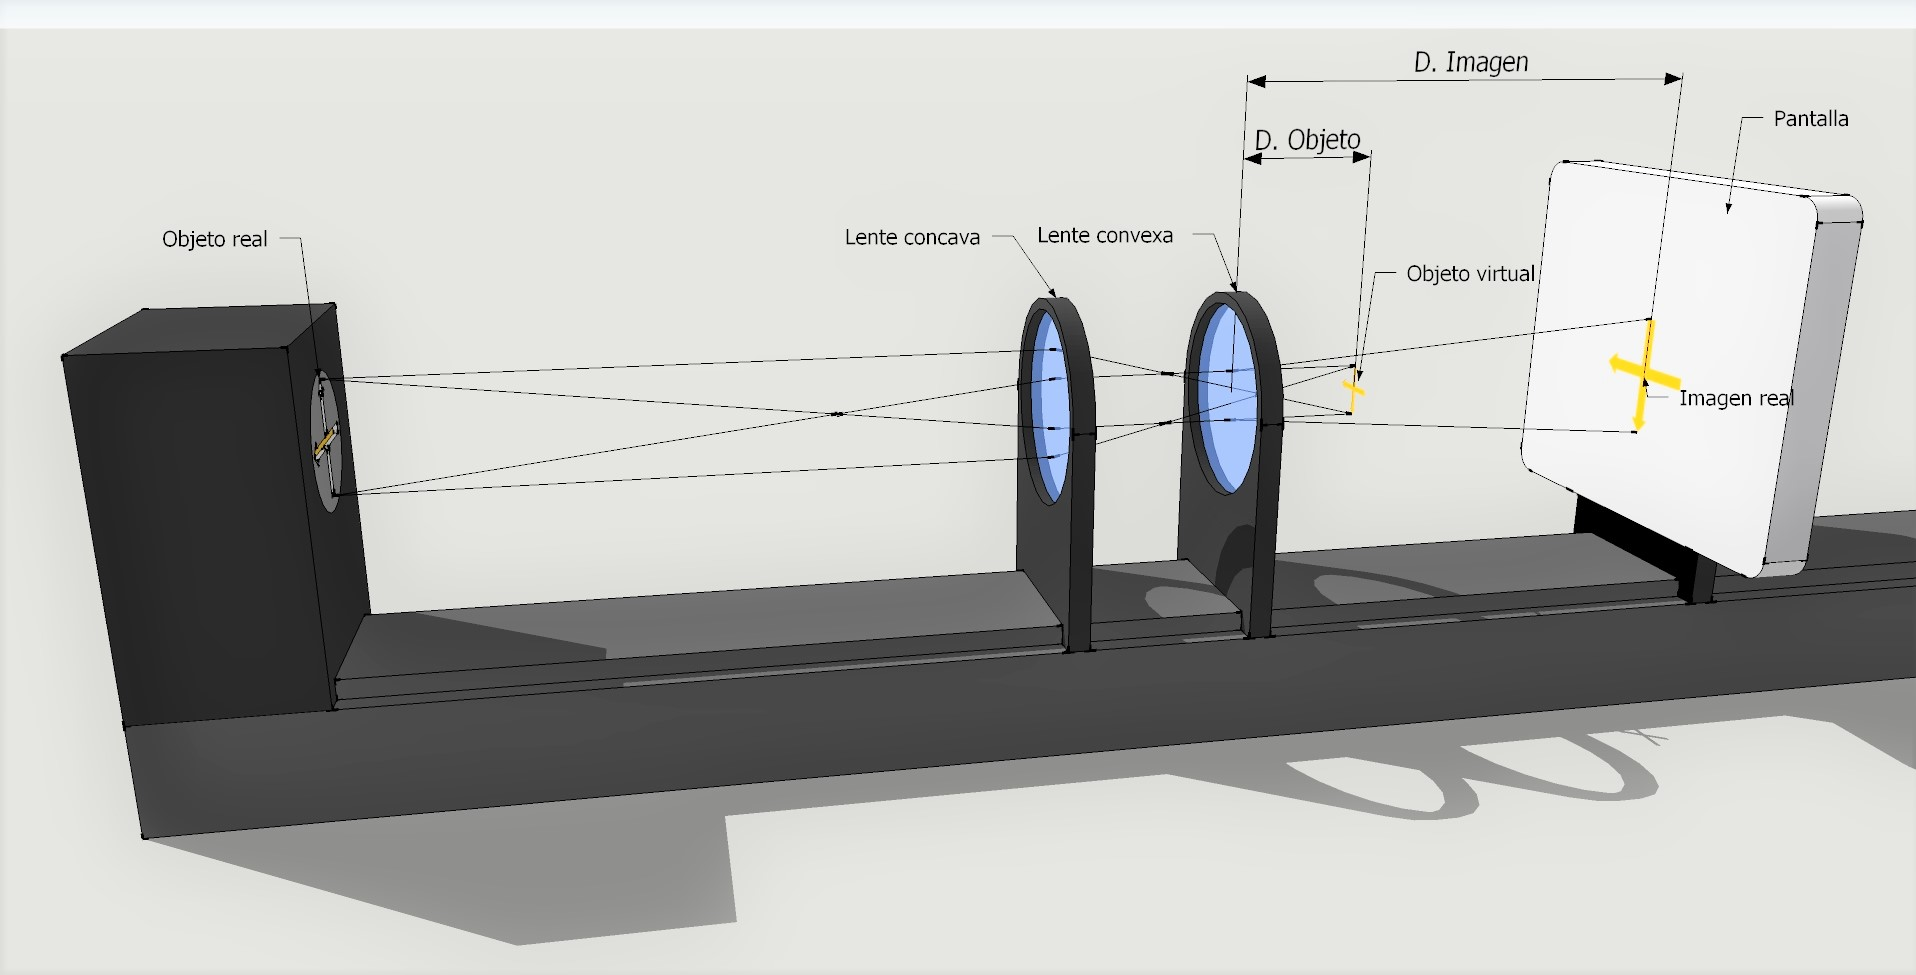
\includegraphics[width=1\linewidth]{DLCX}
            \captionof{figure}{Diagrama experimental de la lente divergente}
            \label{fig:Diagramaconvex}
        \end{Figure}

        En la figura también se aprecia las distancia imagen (\emph{i}) y objeto (\emph{o}) que deseamos medir. Comenzamos ubicando la lente convergente y midiendo la posición de la imagen formada, la cual utilizaremos como \emph{objeto virtual} para la lente divergente, a esta ultima la colocamos un poco antes del objeto virtual, luego comenzamos a moverla hasta que observemos que se forma la imagen en la pantalla. Una vez ubicada la posición donde la imagen es nítida, procedemos a medir la distancia de la pantalla a la lente divergente. Las mediciones se realizan de manera directa utilizando la escala horizontal ubicada sobre el riel que se observa en la figura \ref{fig:Diagramaconvex},a la hora de ubicar la posición de las imágenes reales de las lentes sea ha de considerar un intervalo de longitud en el cual la imagen es nítida y no un único punto. Finalmente 
        Para los siguientes puntos simplemente desplazamos la lente divergente (sin sobrepasar al objeto virtual), encontrando las imágenes en la pantalla, y midiendo las distancias.

    \subsection*{Anteojo astronómico y terrestre}

        El telescopio de Kepler ...

\section*{Datos y resultados}

    \subsection*{Lente convergente}

        Las mediciones para la lente convergente son las mostradas en las tablas \ref{i vs o lc} y \ref{1/i vs 1/o lc}, donde como previamente mencionado en el desarrollo experimental, se fue variando la posición de la lente convergente (y por lo tanto la distancia objeto), y se determinó dónde está la imagen. Si el modelo es aplicable, deberíamos de poder ver una relación lineal entre las inversas de estos valores de la forma:

        \begin{equation*}
            \frac{1}{i} = \frac{1}{f} - \frac{1}{o}
        \end{equation*}

        Por lo que la pendiente de la gráfica debe ser -1 dentro del error, y la ordenada será la inversa de la distancia focal de la lente.

        El error de la distancia objeto es el error de apreciación a la hora de medir la posición de la fuente luminosa y la lente convergente. El error de la distancia imagen es la suma de los errores de apreciación de la fuente y la pantalla, y el error de definición que se tomó como la mitad del intervalo de nitidez de la imagen.

        % Tabla i vs o lente convergente
        \begin{Figure}
            \centering

            \begin{tabular}{cc}
                \toprule
                \textit{\textbf{o $\pm$ $\Delta$o [mm]}} & \textit{\textbf{i $\pm$ $\Delta$i [mm]}}\\
                \midrule
                $200 \pm 2$ & $193 \pm 8$ \\ 
                $300 \pm 2$ & $148 \pm 5$ \\ 
                $400 \pm 2$ & $133 \pm 4$ \\ 
                $500 \pm 2$ & $125 \pm 4$ \\ 
                $600 \pm 2$ & $120 \pm 4$ \\ 
                $700 \pm 2$ & $116 \pm 4$ \\ 
                $800 \pm 2$ & $113 \pm 4$ \\    
                $900 \pm 2$ & $113 \pm 4$ \\ 
                $1000 \pm 2$ & $112 \pm 4$ \\ 
                \bottomrule
            \end{tabular}

            \captionof{table}{i vs o para lente convergente}
            \label{i vs o lc}
        \end{Figure}

        % Tabla 1/i vs 1/o lente convergente
        \begin{Figure}
            \centering

            \begin{tabular}{cc}
                \toprule
                \textit{\textbf{$\frac{1}{o}$ $\pm$ $\frac{\Delta o}{o^2}$ [$mm^{-1}$]}} & \textit{\textbf{$\frac{1}{i}$ $\pm$ $\frac{\Delta i}{i^2}$ [$mm^{-1}$]}}\\
                \midrule
                $0,00500 \pm 0,00005$ & $0,0052 \pm 0,0002$ \\ 
                $0,00333 \pm 0,00002$ & $0,0068 \pm 0,0002$ \\ 
                $0,00250 \pm 0,00001$ & $0,0075 \pm 0,0002$ \\ 
                $0,002000 \pm 0,000008$ & $0,0080 \pm 0,0003$ \\ 
                $0,001667 \pm 0,000006$ & $0,0083 \pm 0,0003$ \\ 
                $0,001429 \pm 0,000004$ & $0,0086 \pm 0,0003$ \\ 
                $0,001250 \pm 0,000003$ & $0,0088 \pm 0,0003$ \\ 
                $0,001111 \pm 0,000002$ & $0,0088 \pm 0,0003$ \\ 
                $0,001000 \pm 0,000002$ & $0,0089 \pm 0,0003$ \\
                \bottomrule
            \end{tabular}

            \captionof{table}{1/i vs 1/o para lente convergente}
            \label{1/i vs 1/o lc}
        \end{Figure}

        \begin{Figure}
            \centering
            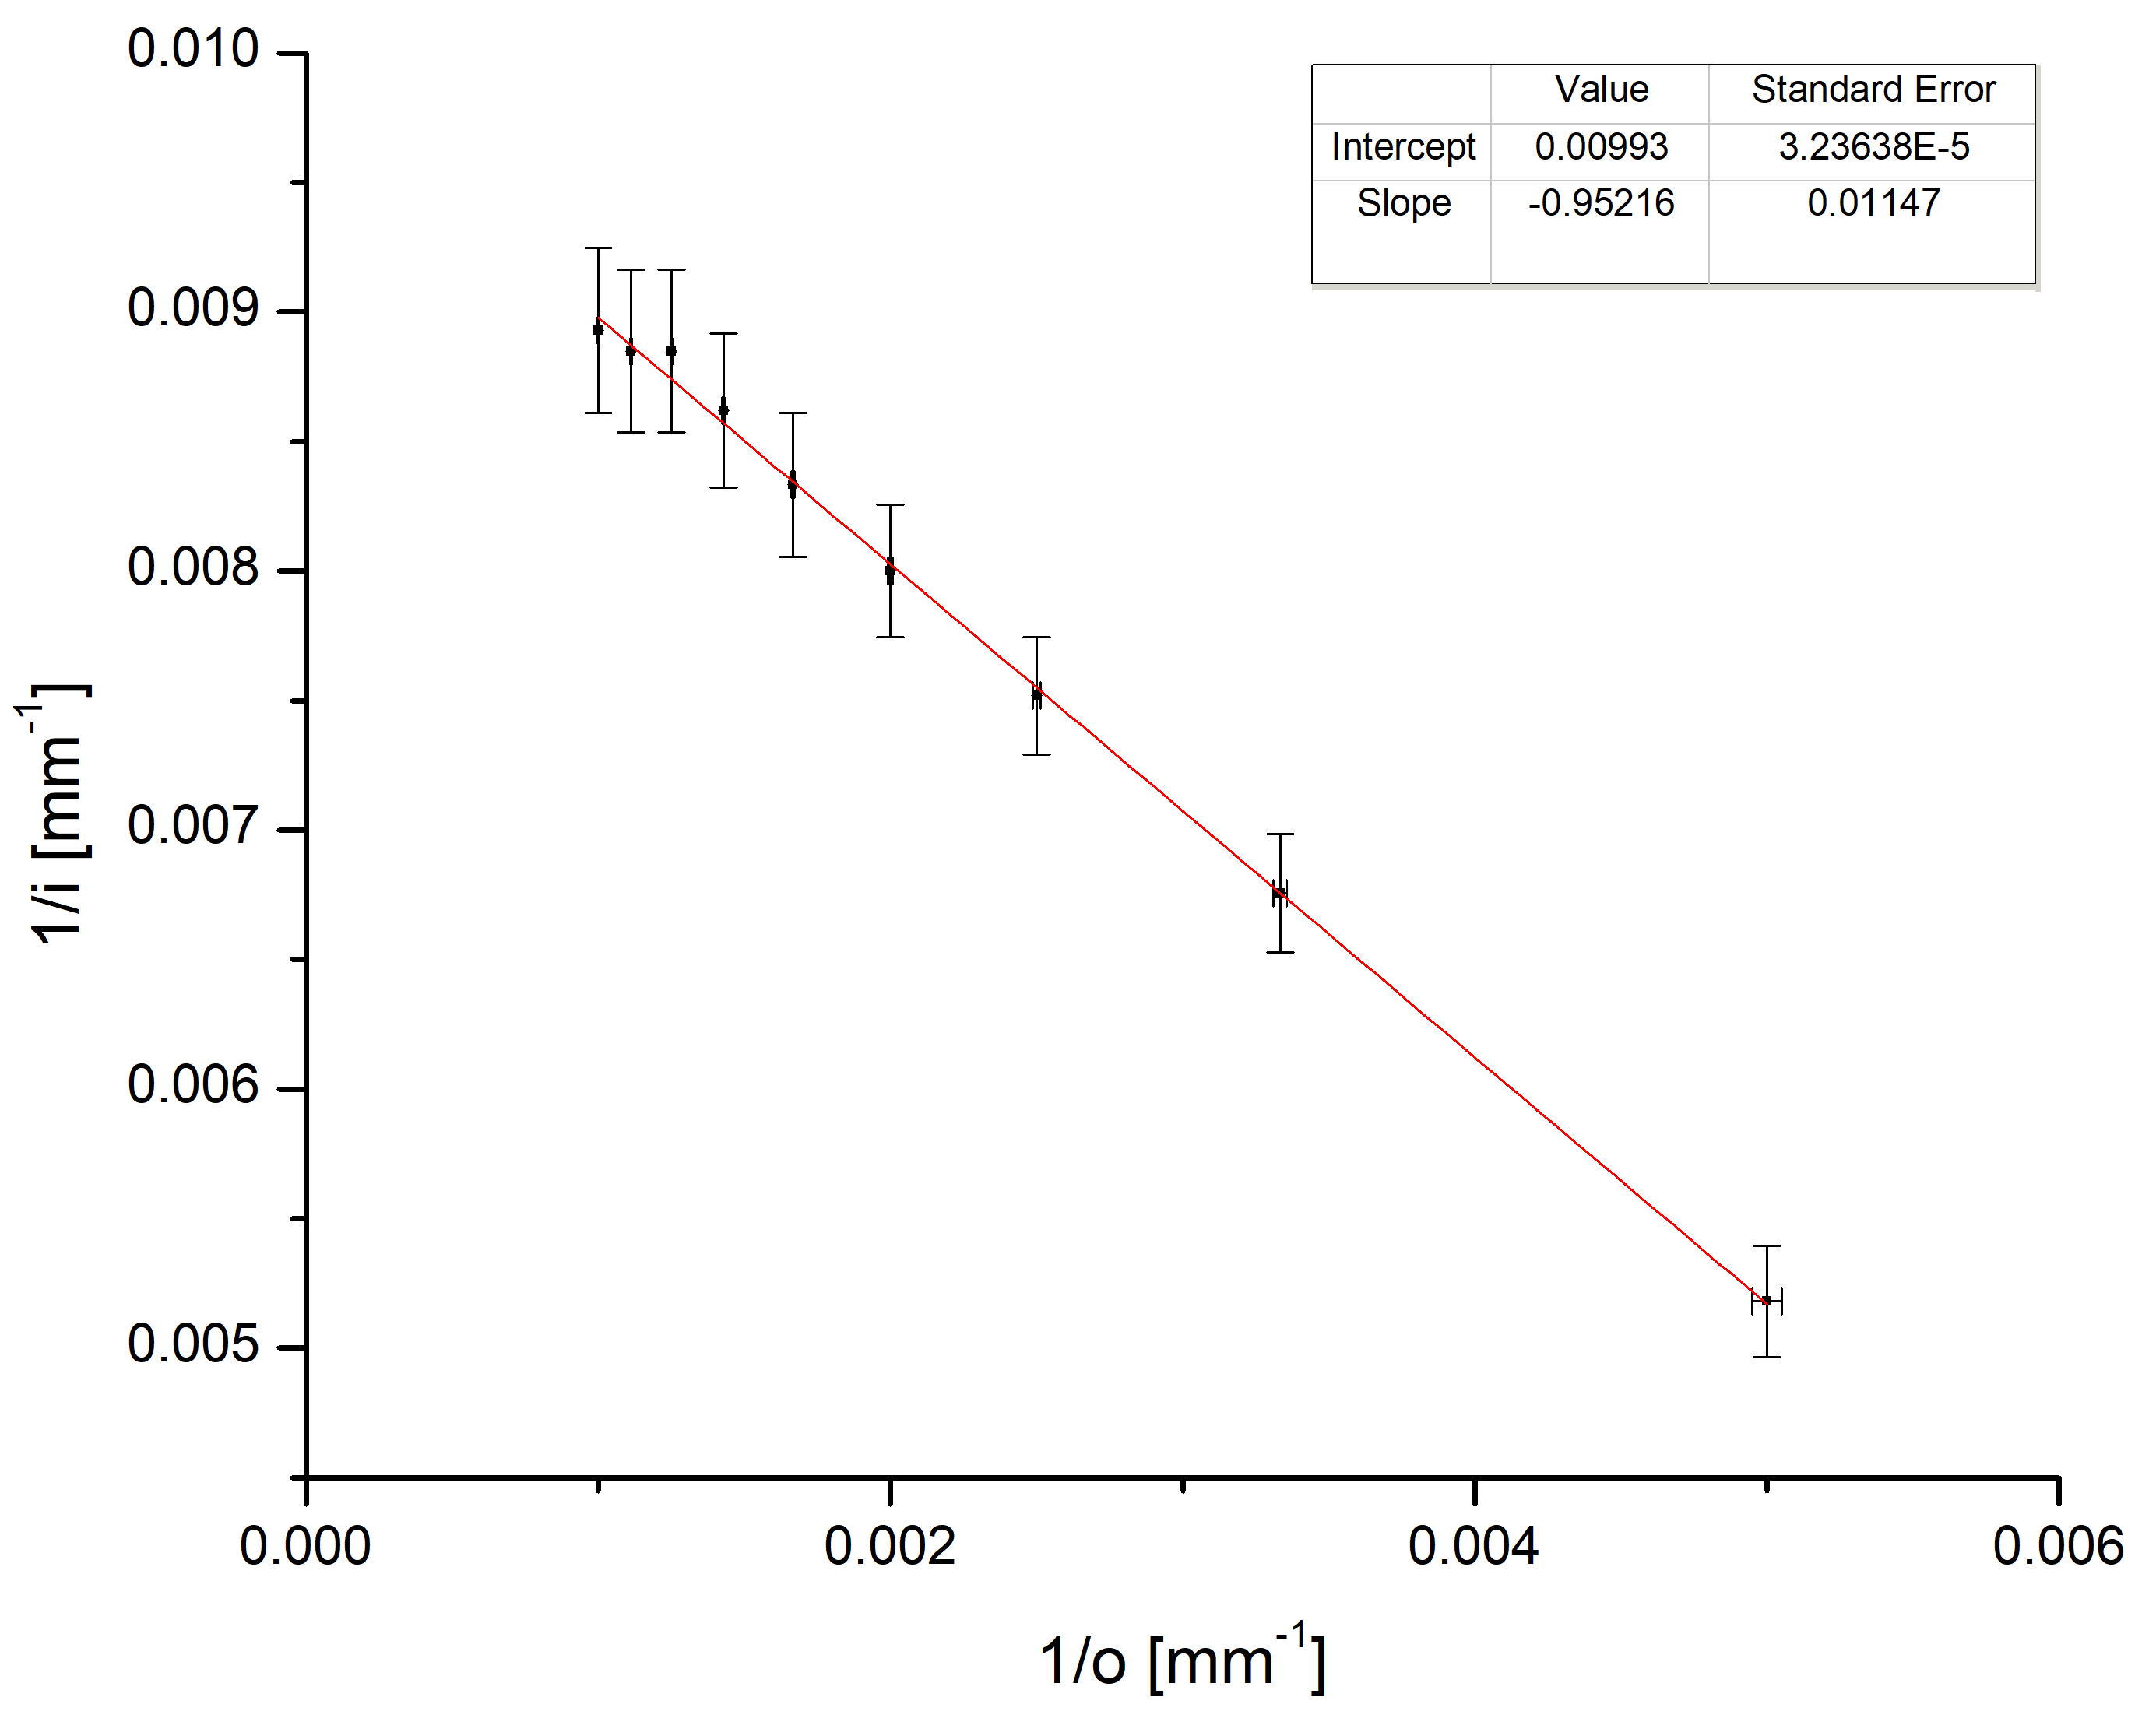
\includegraphics[width=1\linewidth]{Grafica LC.png}
            \captionof{figure}{1/i vs 1/o para lente convergente}
            \label{grafica lc}
        \end{Figure}

        Los parámetros de la recta calculados con el método de cuadrados mínimos, y con el error siendo la suma de dicho método y del método gráfico son:

        Pendiente: $(-0.95$ $\pm$ $0.1)$

        Ordenada: $(9.9$ $\pm$ $0.3)$ . $10^{-3}$ $mm^{-1}$

    \subsection*{Lente divergente}

        Los resultados de las mediciones del sistema de la lente divergente se encuentran colocados en la tabla \ref{tab:Datosdivnor}, todas las mediciones fueron acotadas con 1 mm de apreciación y para aquellas relacionadas con las imágenes de las lentes se les agrego un error de definición el cual consiste en la mitad del intervalo de nitidez mencionado anteriormente en el desarrollo experimental. Los valores de la tabla \ref{tab:Datosdiverinv} se encuentran graficados en la figura \ref{fig:Lentediv}.

        %NORMALES LENTE DIVERGENTE
        \begin{Figure}
            \centering

            \begin{tabular}{cc}
                \toprule
                \multicolumn{1}{c}{\textit{\textbf{o [mm]}}} & \textit{\textbf{i [mm]}} \\
                \midrule
                $(123 \pm 5)$ & $(-73 \pm 3)x10 $\\
                $(113 \pm 5)$ & $(-48 \pm 2)x10$ \\
                $(103 \pm 5)$ & $(-34 \pm 1)x10$ \\
                $(93 \pm 5)$ & $(-251 \pm 4)$ \\
                $(83 \pm 5)$& $(-192 \pm 5)$ \\
                $(73 \pm 5)$ & $(-136 \pm 2)$ \\
                \bottomrule
            \end{tabular}

            \captionof{table}{Distancias objetos e imagen de la lente divergente}
            \label{tab:Datosdivnor}
        \end{Figure} 

        %INVERSOS LENTE DIVERGENTE
        \begin{Figure}
            \centering

            \begin{tabular}{cc}
                \toprule
                \textit{\textbf{1/o [$mm^{-1}$]}} & \textit{\textbf{1/i [$mm^{-1}$]}} \\
                \midrule
                $(0.0082 \pm 0.0003)$ & $(-0.00138 \pm 0.00006)$ \\
                $(0.0089 \pm 0.0004)$ & $(-0.00208 \pm 0.00009)$ \\
                $(0.0097 \pm 0.0005)$ & $(-0.00293 \pm 0.00009)$ \\
                $(0.0108 \pm 0.0006)$ & $(-0.00399 \pm 0.00009)$ \\
                $(0.0121 \pm 0.0007)$ & $(-0.0052 \pm 0.0002)$ \\
                $(0.0137 \pm 0.0009)$ & $(-0.0074 \pm 0.0002)$ \\
                \bottomrule 
            \end{tabular}

            \captionof{table}{Inversos de o e i para la lente divergente}
            \label{tab:Datosdiverinv}
        \end{Figure}

        \begin{Figure}
            \centering
            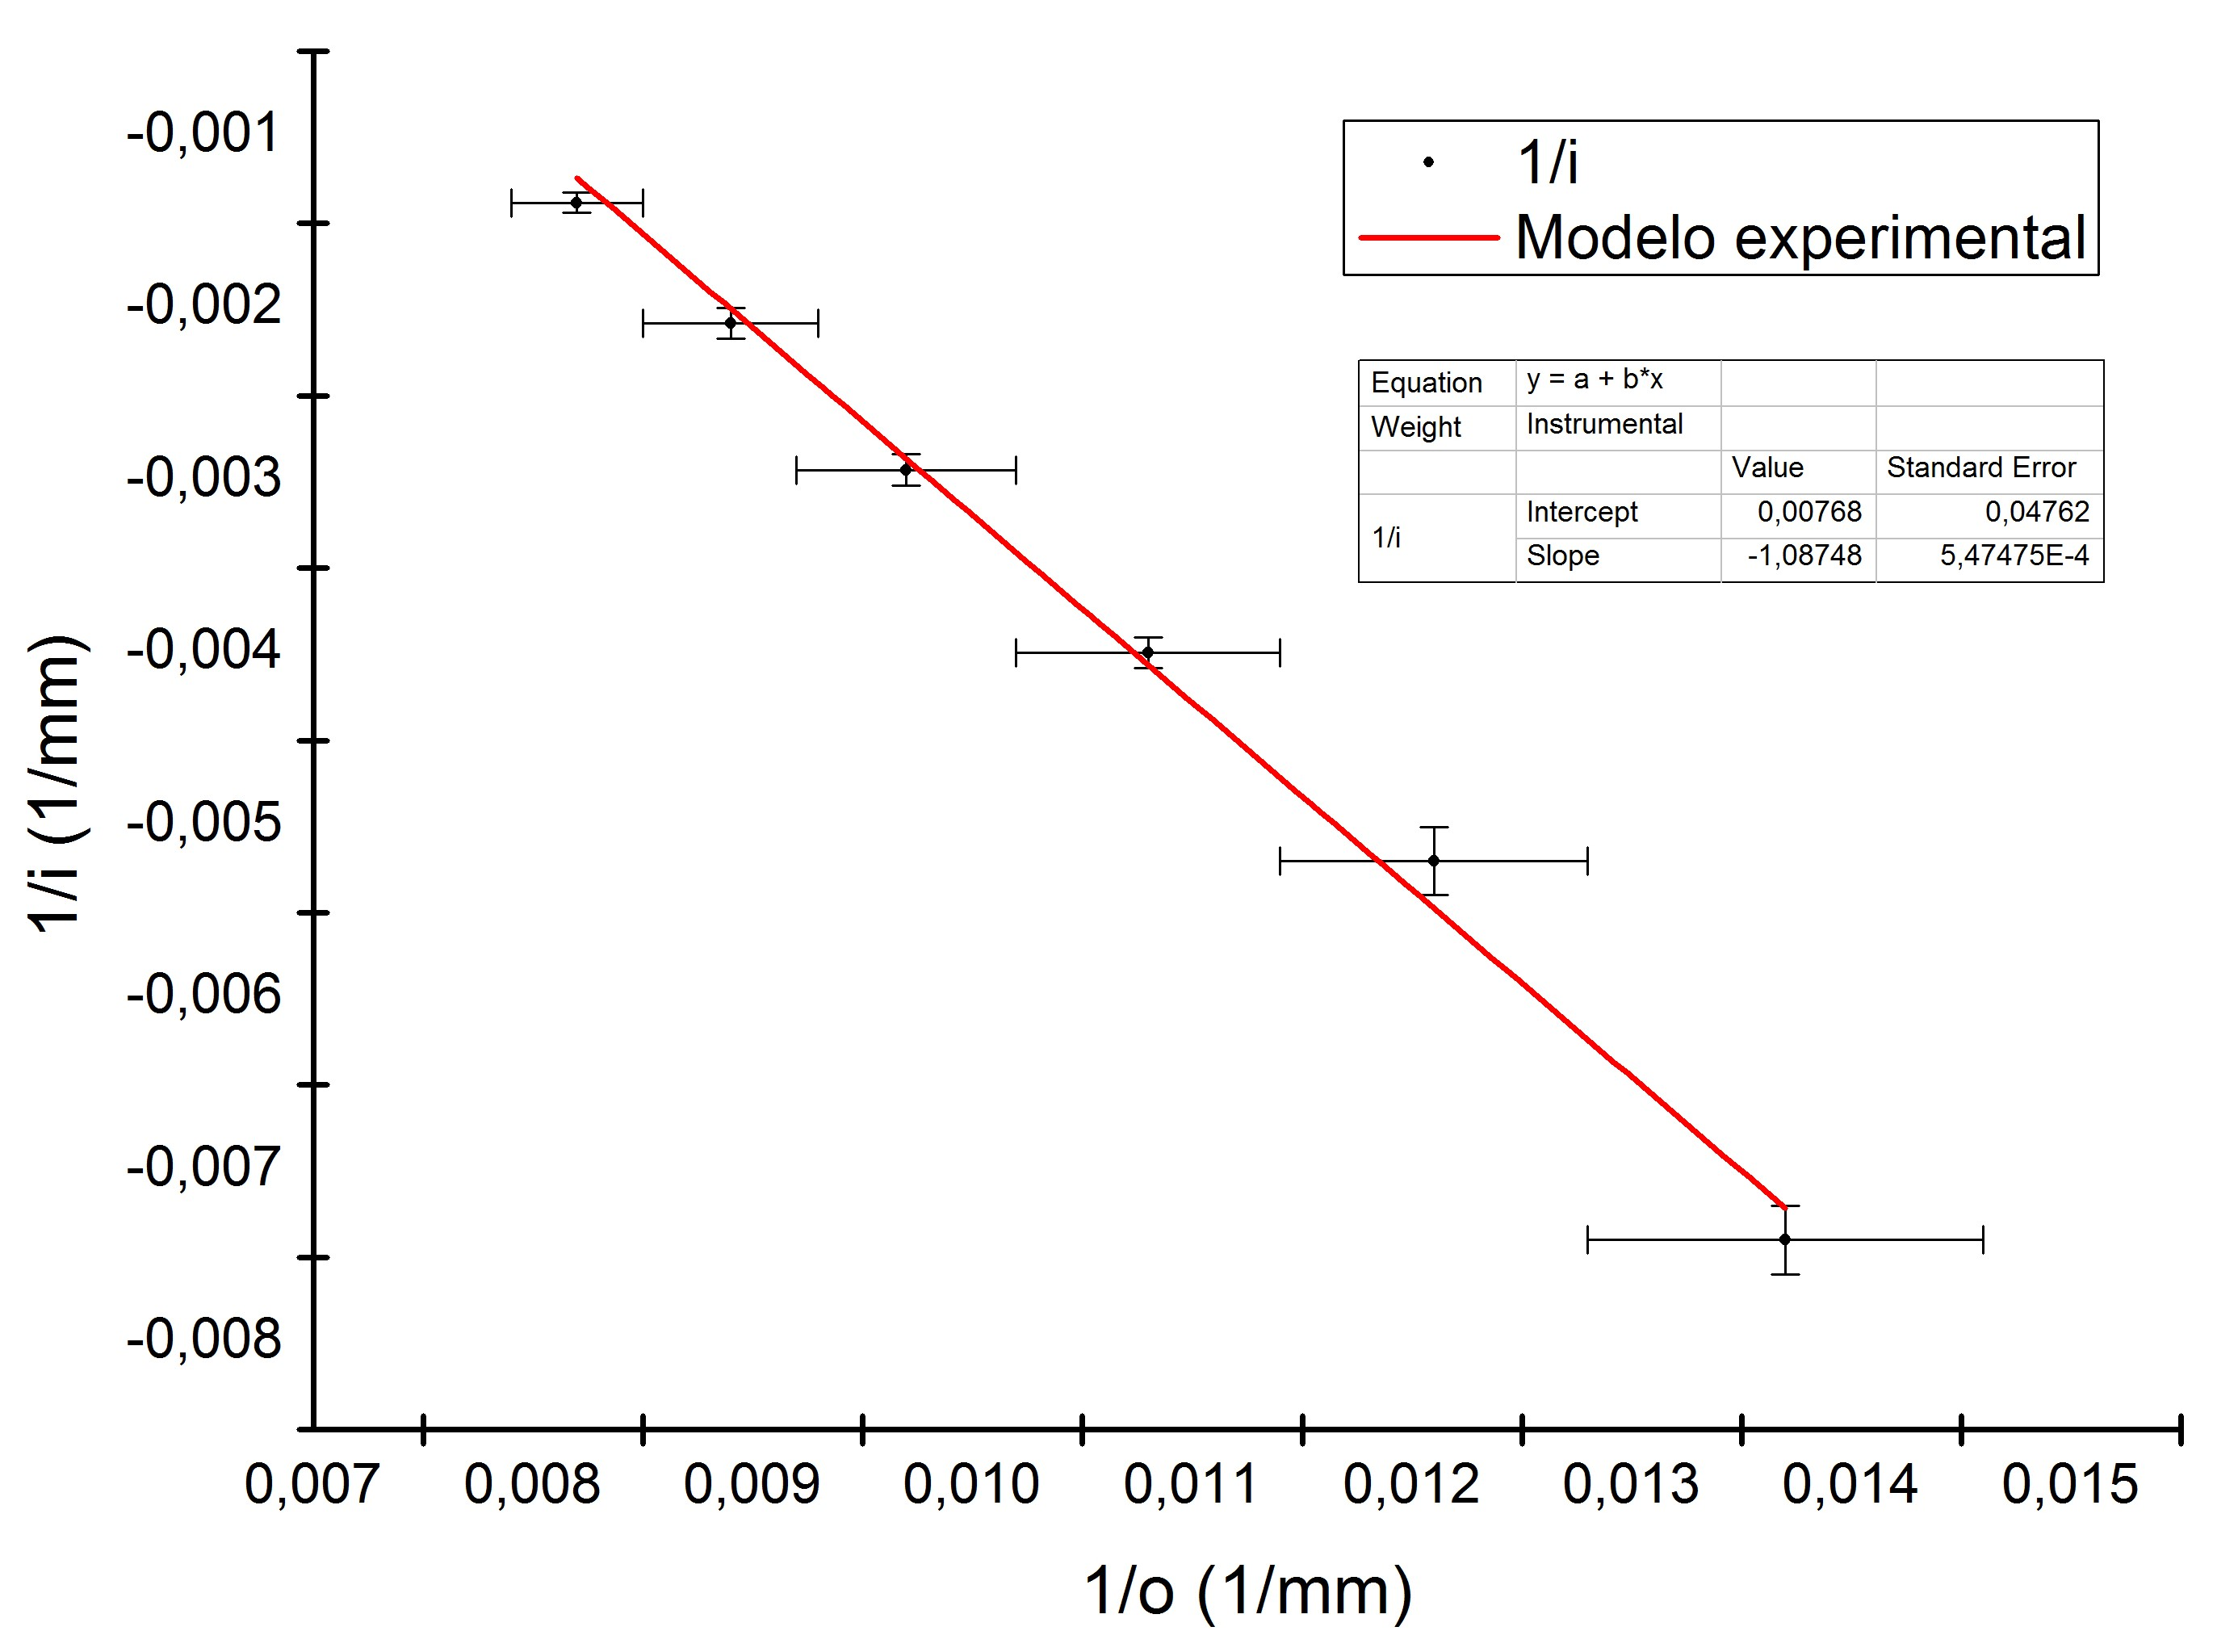
\includegraphics[width=1\linewidth]{Lente divergente.jpg}
            \captionof{figure}{Grafica de $i^{-1}$ vs $o^{-1}$ para la lente divergente}
            \label{fig:Lentediv}
        \end{Figure}

        Los parámetros de la recta calculados con el método gráfico son: 

        Pendiente: $A=(-1,1$ $\pm$ $0,2)$

        Ordenada: $B=(0,008$ $\pm$ $0,001)$ $mm^{-1}$

        Tanto la grafica de la figura \ref{fig:Lentediv} como la pendiente de la recta corresponden con el comportamiento que predice el modelo en , luego podemos asignar a la ordenada al origen la relación: $B=1/f$ y determinar la distancia focal de la lente, su valor acotado es: $f=(1,3$ $\pm$ $0,1)$ . $10^{2}$ $mm$.
 
    \subsection*{Control de supuestos}

        Para verificar si en nuestro diseño experimental son o no apreciables las aberraciones de esfericidad (Fig. \ref{f:abesf}) o cromáticas (Fig. \ref{f: abcro}), controlamos los supuestos con los siguientes sistemas experimentales:

        \begin{itemize}
            \item Para las \emph{aberraciones de esfericidad} utilizamos dos diafragmas, figura \ref{f: Dparax} y figura \ref{f: Dmarg}, que interfieren el camino óptico de los rayos paraxiales y de los rayos rayos marginales respectivamente.
            \item Para las \emph{aberraciones cromáticas} utilizamos dos acetatos, uno de color rojo y otro de color azul, para utilizar un espectro mas acotado de la luz visible.
        \end{itemize}

        %diafragmas
        \begin{Figure}
            \centering
            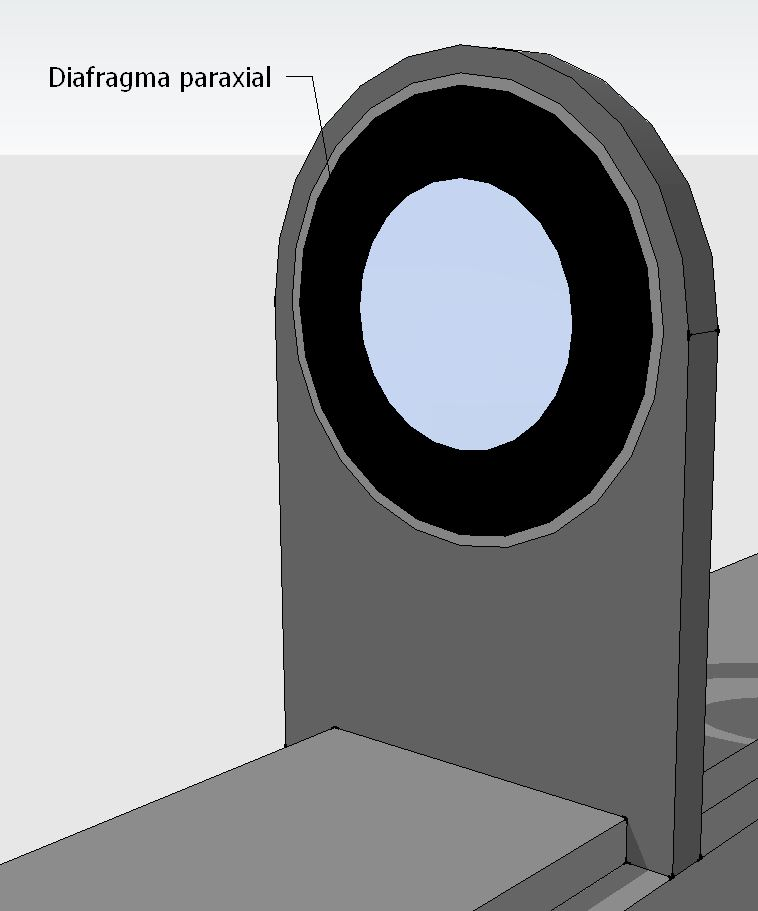
\includegraphics[width=0.7\linewidth]{Diafragma paraxial.JPG}
            \captionof{figure}{Diafragma paraxial}
            \label{f: Dparax}
        \end{Figure}

        \begin{Figure}
            \centering
            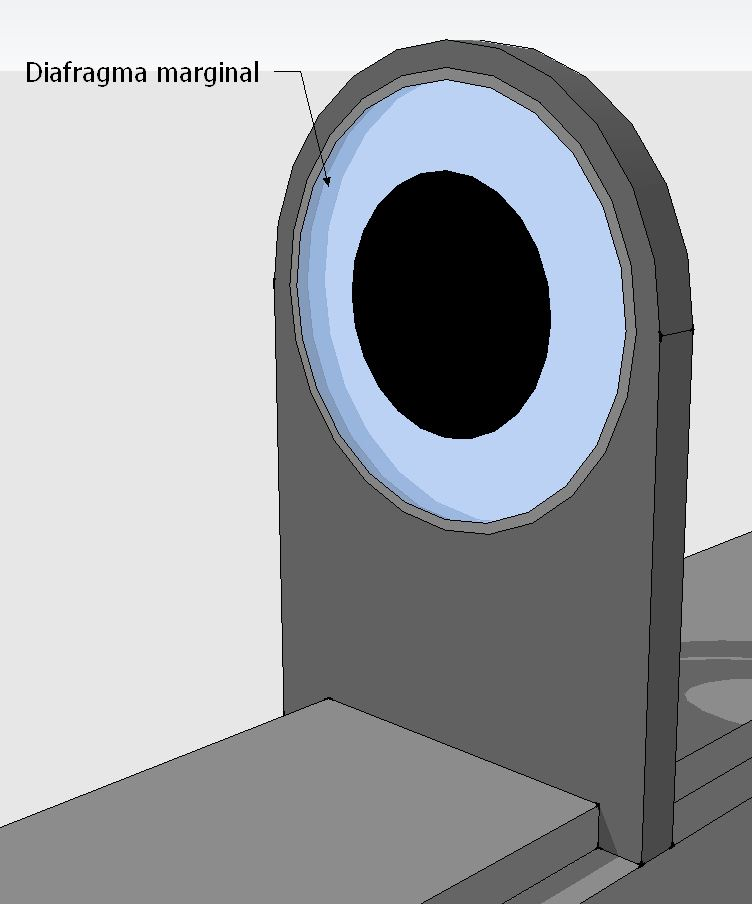
\includegraphics[width=0.7\linewidth]{Diafragma marginal.JPG}
            \captionof{figure}{Diafragma marginal}
            \label{f: Dmarg}
        \end{Figure}

        Recogemos los datos de la distancia imagen y la distancia objeto con una lente convergente en la tabla \ref{tab:supuestos}.

        Las aberraciones de esfericidad y cromáticas van a ser despreciables si se cumple la siguiente relación:

        \begin{equation}
            \centering
            \Delta f_{b} + \Delta f_{a} \geq f_{b} - f_{a}
        \end{equation}
 
        \begin{Figure}
            \centering

            \begin{tabular}{c|c c}
                \toprule
                 & \textit{Distancia objeto} & \textit{Distancia imagen}\\
                 & \textit{$[mm]$} & \textit{$[mm]$}\\
                \midrule
                Control & $(256 \pm 7)$ &$(183 \pm 8)$\\ \hline
                Diafragma & \multirow{2}{*}{$(263 \pm 2)$} & \multirow{2}{*}{$(187 \pm 3)$}\\
                paraxial & & \\
                Diafragma & \multirow{2}{*}{$(256 \pm 8)$} & \multirow{2}{*}{$(19 \pm 1)\times 10$}\\
                periferico & & \\ \hline
                Rojo & $(255 \pm 6)$ &$(186 \pm 7)$\\
                Azul & $(253 \pm 5)$ &$(187 \pm 6)$\\ 
                \bottomrule
            \end{tabular}

            \captionof{table}{Control de supuestos}
            \label{tab:supuestos}
        \end{Figure}

\section*{Conclusiones}

    \subsection*{Lente convergente}

        Como el valor de la pendiente está dentro de lo esperado por el modelo, y la recta se ajusta a los datos, podemos calcular la distancia focal de la lente, y nos da:

        f = $(101$ $\pm$ $3)$ mm

        La distancia focal de la lente dada por el fabricante es de 100 mm, con un mínimo error de 1 mm. La distancia focal calculada es la misma dentro del error.

    \subsection*{Lente divergente}
    
        
    
    \subsection*{Control de supuestos}
    
        

\begin{thebibliography}{99}

    \bibitem{1} Sears, Zemansky. \emph{Física universitaria}, vol. 2, 14th ed. Pearson Education, 2018.

    

\end{thebibliography}

\end{multicols*}

\end{document}